\newpage
\section{XDDCP}\label{xddcp}

Xddcp is a shell script located in the ``contrib'' subdirectory of the standard XDD distribution. This shell script is used to copy one or more files from one computer to another over a network. It is intended to be used for very large files, typically in excess of 50 Gigabytes each, over high-speed networks starting at 10Gigabits/sec. Figure XX illustrates the basic operation of XDDCP.

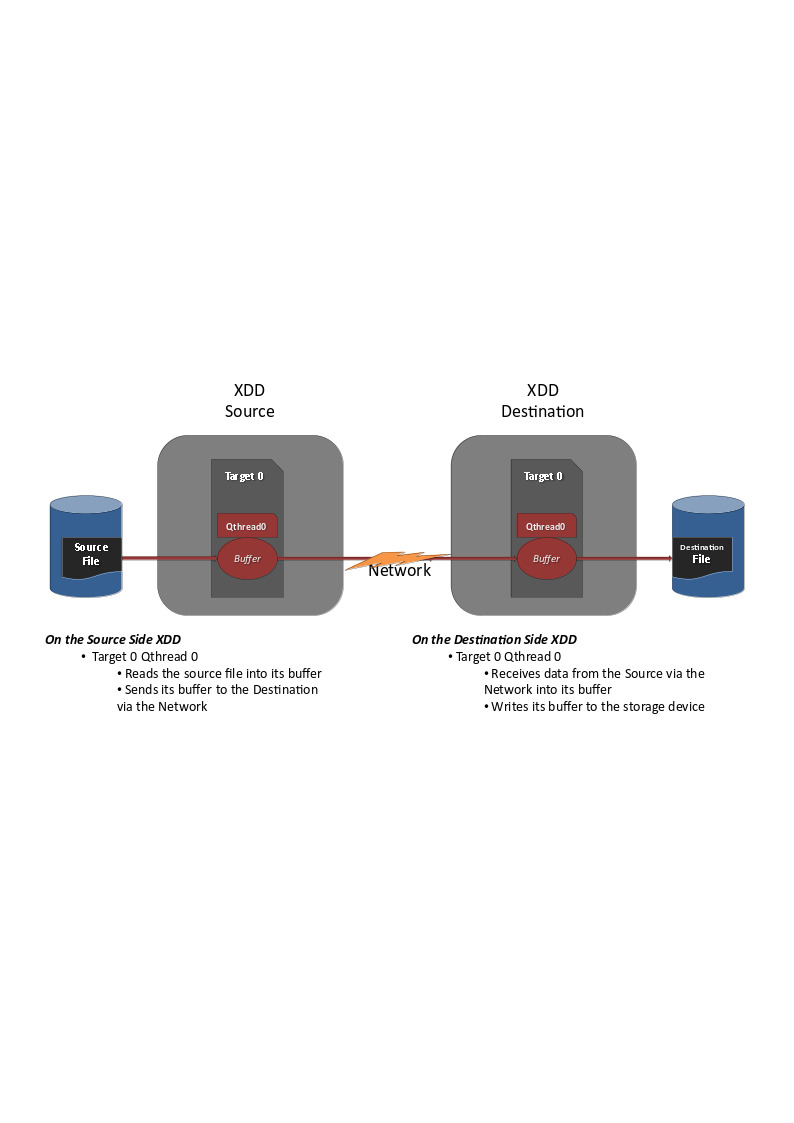
\includegraphics[width=7in,height=3.47917in,alt={Slide1.JPG}]{./images/media/image4.jpg}

Xddcp uses xdd and the End-to-End option to accomplish the data copy operation. It does this by starting an instance of XDD on the ``destination'' computer using ssh and then starting an instance of XDD on the ``source'' computer. The ``source'' side is defined to be where the original file exists. The ``destination'' side is defined to be where the copy of the file will be created.

The destination side is started first and ``listens'' on the specified socket numbers. This version of XDD requires a unique socket number for each ``QThread Pair''. A QThread Pair consists of a source side QThread that sends data to a corresponding destination side QThread through a specific port number.

\subsection{XDDCP Usage}\label{xddcp-usage}

\textbf{xddcp} \emph{{[}OPTIONS{]}} source\emph{\_file destination\_host:destination\_file {[}size{]}}

\begin{quote}
\emph{source\_file} - complete /filepath/name for source file on source host

\emph{destination\_host} - destination host IP or Name over which data is transferred

\emph{destination\_file} - complete /filepath/name for destination file on destination host

\emph{size} - number of bytes to transfer {[}Default: size of source file{]}
\end{quote}

\textbf{\ul{OPTIONS}}

--\textbf{a} -- Specifies that this invocation of xddcp should keep a restart file so that the copy operation can be resumed at a later time if it is interrupted. If this is the resumption of a prior invocation of xddcp then it is used to resume a transfer from the point where the previous invocation was interrupted.

--\textbf{d} -- Use Direct I/O on the destination side of the copy.

--\textbf{s} -- Use direct I/O on the source side of the copy.

--\textbf{f} -- If ports are unavailable on destination, attempt to kill any running XDD's that are running on the destination side and retry starting the destination-side XDD.

--\textbf{F} -- Transfer a list of files named in \emph{source\_file} which is a simple ASCII text file with one file name per line. File names can be either relative or fully qualified path names.

--\textbf{h} -- Print out usage information.

--\textbf{p} \emph{portnum} -- First port to use for transfer {[}Default: 40010{]}. This is also known as the base port.

--\textbf{o} -- Ordered-mode, write data in serial order on the destination side. Normally, no ordering is used on the destination side.

--\textbf{t} \emph{threads} -- Used to specify the number of QThreads to use on the source and destination sides of a copy operation. {[}Default: 8{]}

--\textbf{v} -- Additional information added to the output log files. This will also cause timestamp files to be generated on both the source and destination sides of a copy.

--\textbf{w} -- Same as the --v option but will also generate a binary tim

\textbf{NOTE:} \textquotesingle xdd.Linux\textquotesingle{} must be in your PATH env on both source and destination hosts

\subsection{End-to-End and XDDCP Theory of Operation}\label{end-to-end-and-xddcp-theory-of-operation}

XDDCP uses the End-to-End options to accomplish the task of copying data from one computer to another over a network. The End-to-End operation is accomplished by a ``matched pair'' of XDD instances with one instance running on the ``Source'' computer and the other instance running on the ``Destination'' computer. The ``Source'' computer is defined to be the system that reads in the original file and transmits its contents over a network to the ``Destination'' computer which is defined to be the system that writes the copy of the file to stable storage. Data movement is always from the Source to the Destination.

It is important to note that the Source and Destination instances of XDD must be ``matched'' in the sense that they each have the same queue depth and that they agree on which network addresses and ports to use. For E2E operations the queue depth can either be specified explicitly using the ``-queuedepth'' option or it can be specified implicitly using the ``\textbf{-e2e destination} \emph{hostname:base\_port,number\_of\_ports}'' option. When the queue depth is specified implicitly, it will take precedence over the ``-queuedepth'' option if it is also specified. Furthermore, the queue depth implied on the \textbf{``-e2e destination\ldots''} option is the sum of all ``number\_of\_ports'' specified for a given XDD run.

For example,

The following diagram describes how E2E works with multiple threads:

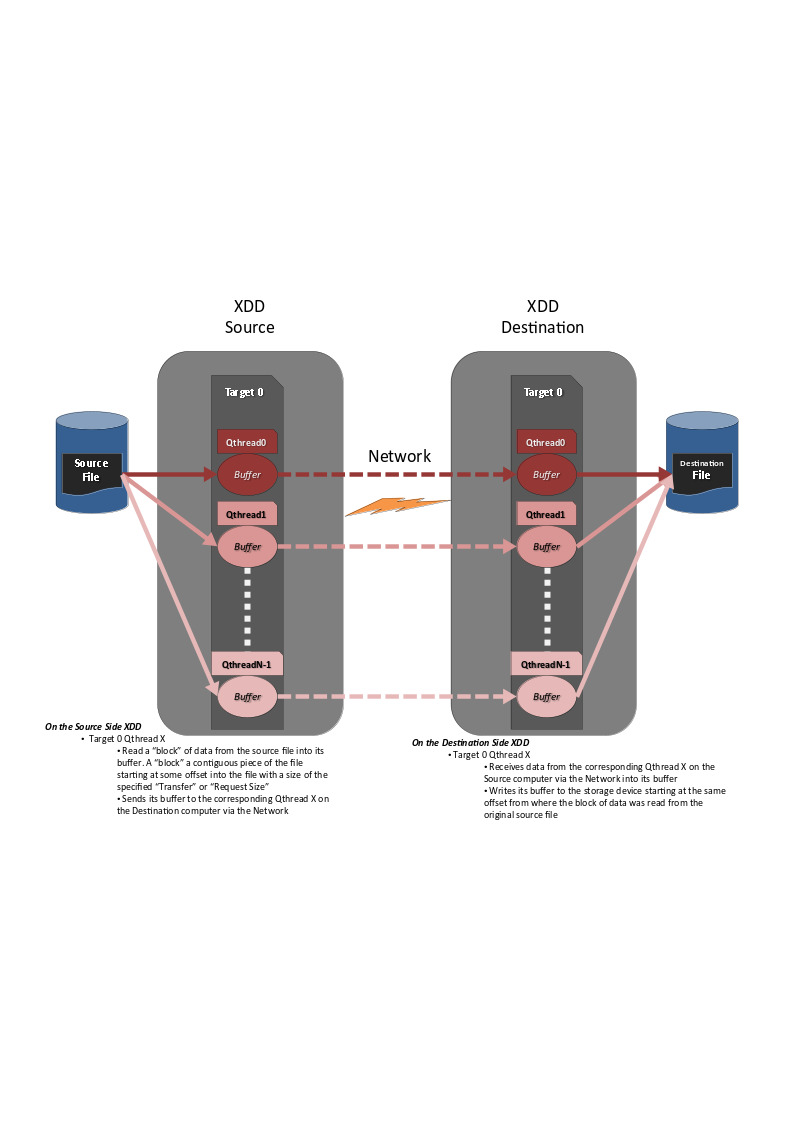
\includegraphics[width=7in,height=5.26736in,alt={Slide2.JPG}]{./images/media/image5.jpg}

XDD can use either buffered I/O or Direct I/O for reading the source file or writing the destination file. Buffered I/O will increase the CPU overhead and possibly result in lower overall bandwidth performance of an E2E operation. Therefore, it is recommended that Direct I/O be used whenever possible. The following diagrams illustrate the basic difference between buffered I/O and Direct I/O as they relate to an E2E operation.

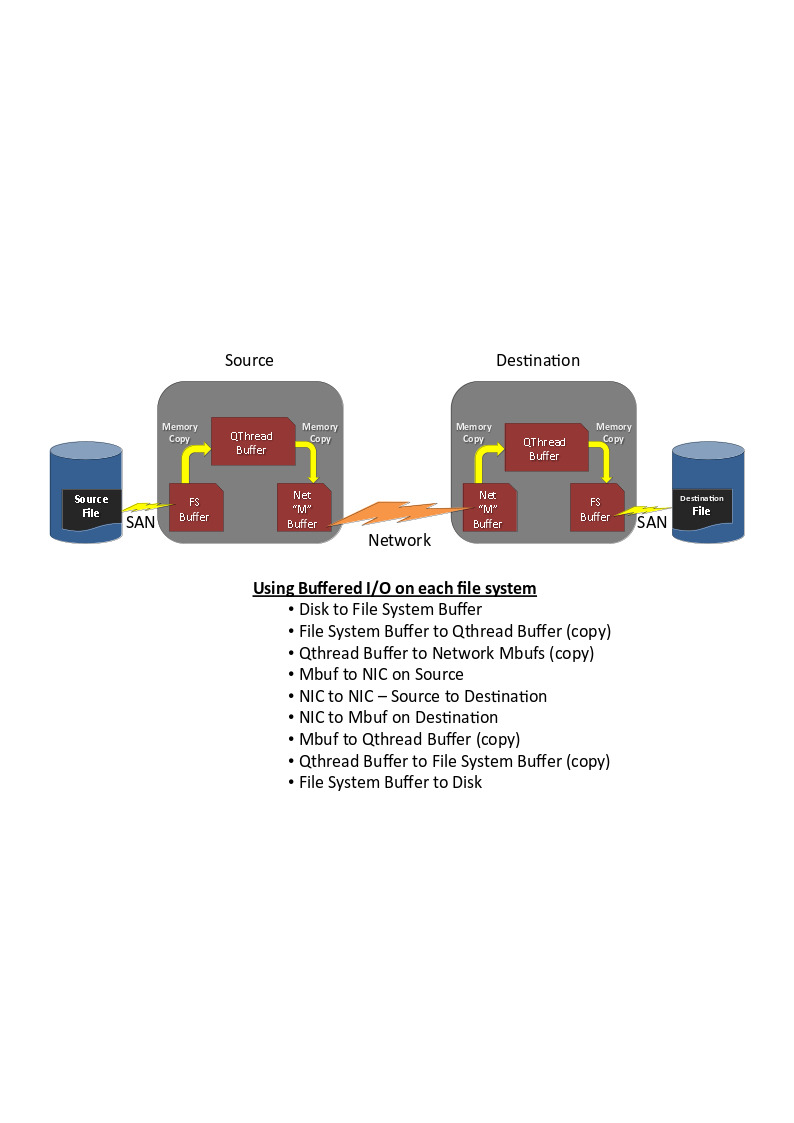
\includegraphics[width=7in,height=4.41667in,alt={Slide3.JPG}]{./images/media/image6.jpg}

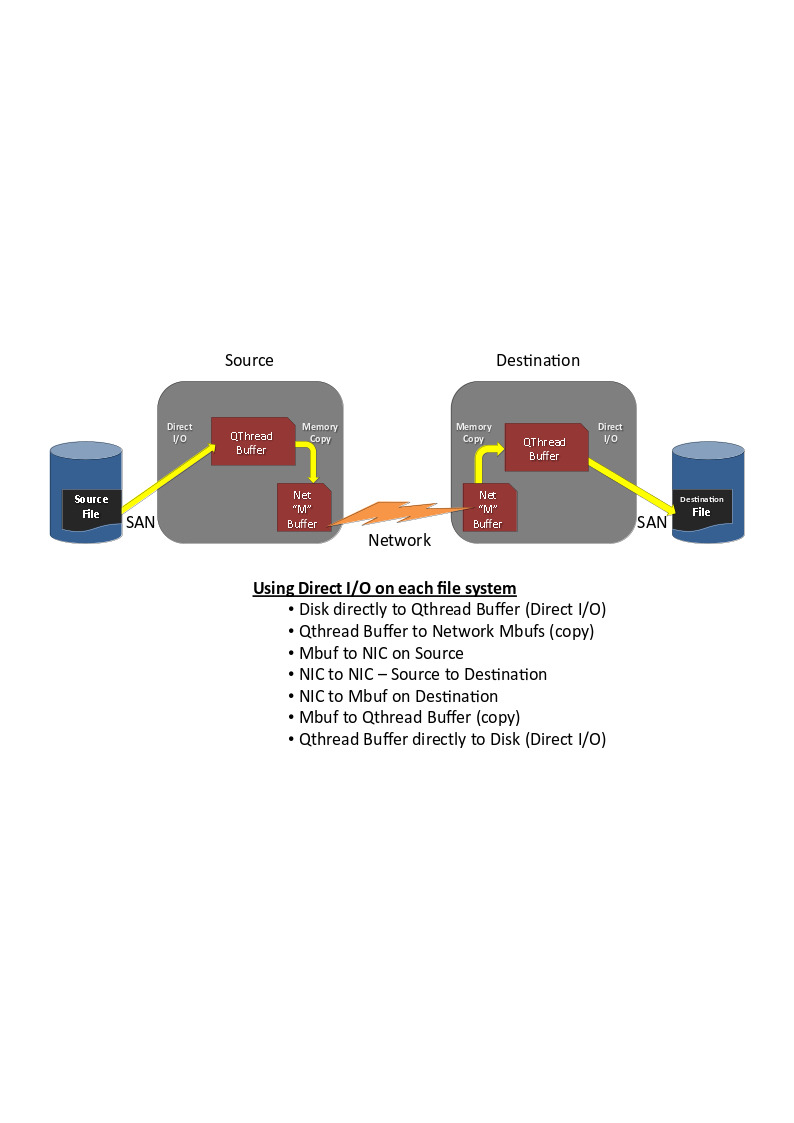
\includegraphics[width=7in,height=4.03125in,alt={Slide4.JPG}]{./images/media/image7.jpg}

